%% Figure from MATH 556 notes, section 48 (Lecture 21). ADDED (not from lecture).
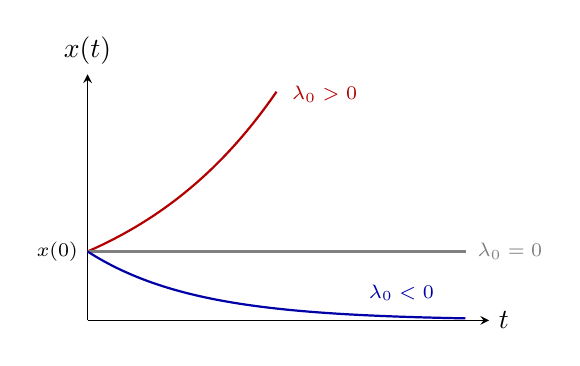
\begin{tikzpicture}[>=stealth, xscale=1.5, yscale=1.25]
    \draw[->] (0,0) -- (3.4,0) node[right] {$t$};
    \draw[->] (0,0) -- (0,2.5) node[above] {$x(t)$};
    \draw[thick, red!70!black, domain=0:1.6, samples=40, smooth] plot (\x, {0.7*exp(0.75*\x)});
    \draw[thick, gray, domain=0:3.2, samples=2] plot (\x, {0.7});
    \draw[thick, blue!65!black, domain=0:3.2, samples=40, smooth] plot (\x, {0.7*exp(-1.1*\x)});
    \node[left, font=\scriptsize] at (0,0.7) {$x(0)$};
    \node[red!70!black, font=\scriptsize, anchor=west] at (1.65,2.3) {$\lambda_0 > 0$};
    \node[gray, font=\scriptsize, anchor=west] at (3.22,0.7) {$\lambda_0 = 0$};
    \node[blue!65!black, font=\scriptsize, anchor=south west] at (2.3,0.1) {$\lambda_0 < 0$};
\end{tikzpicture}
